\documentclass[12pt, a4paper]{article}
\title{Relazione progetto ROOT} %argomento
\date{}
\author{Stella Baldrati, Giacomo Errani, Riccardo Giuliani}

\setlength{\parindent}{0pt}
\usepackage{setspace}
\usepackage[margin=0.5in]{geometry}
\usepackage{float}
\usepackage{amsfonts}
\usepackage{pdfpages}
\usepackage{verbatim}
\usepackage[utf8]{inputenc}
\usepackage{subcaption}
\usepackage{graphicx}

%\usepackage{siunitx} 
%\sisetup{
  %round-mode          = places, % Rounds numbers
 % round-precision     = 2, % to 2 places
%}

\graphicspath{ {./images} } %cartella immagini, separata dalla cartella files

\usepackage{listings}
\usepackage{xcolor}


\begin{document}

\maketitle

\section{Introduzione}
%%inserire un po' di teoria alla base e sintetizzare tutto il contenuto come in un abstract

L'approccio sperimentale utilizzato in fisica delle particelle per studiarne proprietà e interazioni si basa sullo studio dei prodotti di collisioni ad alta velocità. In seguito a questi urti, si genera un numero di particelle di varie tipologie stimato in $10^2-10^4$ per ogni evento di collisione. 
\newline
Le particelle più stabili sono direttamente rilevabili e si possono classificare tramite analisi della traiettoria. Vi sono però anche particelle instabili, dette risonanze, che decadono in tempi brevissimi e non sono direttamente rilevabili; per studiarle si rende necessario analizzare i prodotti dei loro decadimenti, che generalmente sono particelle sufficientemente stabili.
\newline
Il programma qui illustrato simula eventi di collisione e genera prodotti assimilabili a quelli ottenibili tramite un acceleratore. Analizza poi le particelle generate ed elabora i decadimenti, rappresentandone quantità e distribuzioni tramite grafici ROOT. 

In particolare, consente di studiare il comportamento della risonanza K*, cercandone il picco caratteristico di massa invariante dovuto ai prodotti del suo decadimento nel segnale di fondo.

\section{Struttura del codice}
%quali classi sono state implementate, con che funzione,
%quali meccanismi di reimpiego di codice sono stati usati, e perchè

\subsection{Programma di generazione}

Sono state implementate le seguenti classi:

\begin{enumerate}
\item ParticleType: rappresenta una generica particella stabile categorizzandola mediante massa, carica e tipologia, e fornisce un'interfaccia per accedere a questi dati. Implementa inoltre una funzione \verb!GetWidth! che fornisce una larghezza di risonanza nulla, necessaria per poter utilizzare il polimorfismo dinamico. 
Definisce un enum che identifica i tipi di particelle utilizzabili, poi associati alle istanze di ParticleType.

\item ResonanceType: classe derivata di ParticleType, rappresenta il fenomeno di risonanza per una particella instabile con l'attributo larghezza di risonanza e reimplementa \verb!GetWidth! per restituire il valore corretto. 

\item Particle: rappresenta una particella della simulazione, mediante il tipo e la quantità di moto. 
Fornisce dei metodi per accedere agli attributi della particella, per calcolare la massa invariante ed elaborare un decadimento (funzione \verb!Decay2Body!).
Definisce un vettore statico (\verb!fParticleTypes!) che memorizza i tipi di particelle, associati alle singole istanze mediante l'attributo \verb!fParticleName!.

\item ProportionGenerator: class template che implementa il generatore secondo definite proporzioni. 
\item ParticleGenerator: oggetto funzione che incapsula la generazione delle particelle. 
Fornisce un \verb!operator()! per eseguire la generazione e una funzione \verb!loadParticles()! per caricare i parametri dei tipi di particelle nel vettore \verb!fParticleTypes!.

\item ParticleStorage: struct serializzabile che memorizza i vari istogrammi, generata da ParticleGenerator.

\end{enumerate}

\subsection{Programma di analisi}

\begin{enumerate}
\item ParticleAnalyser: incapsula la lettura del file root (con controllo integrità dei dati mediante un cast dinamico) nel costruttore. Fornisce un metodo \verb!GetData! per accedere ai dati, una funzione di analisi dei segnali dei decadimenti (\verb!GetDecaymentSignal!) e una di analisi delle distribuzione di generazione (\verb!GetGenerationFits!). 

\item AnalyserGraphics: incapsula la presentazione dei dati, crea i canvas, configura lo stile, disegna istogrammi e fit.


\end{enumerate}

\subsection{Tecniche di reimpiego del codice}
%note su cosa scrivere: tecniche oop, incapsulamento, uso della classe proportion generator, implementare la funzionalità comune in classi e usando funzioni generiche, nascondendo i dettagli implementativi
Abbiamo usato le tecniche della programmazione OOP per separare dettagli implementativi e interfaccia, incapsulando le funzioni e rendendo il tutto modulare.
\newline

In particolare, la classe \verb!ProportionGenerator! si adatta a generare qualsiasi tipo di oggetto, note le istanze generabili e le probabilità.
\newline

Infine, l'uso del polimorfismo dinamico nelle classi \verb!ParticleType! e \verb!ResonanceType! consente di gestire le particelle stabili e instabili con puntatori di tipo \verb!ParticleType!, trattandole come se fossero dello stesso tipo.

\section{Generazione}
% specifichiamo che si tratta di eventi separati e non tutte insieme

Sono stati elaborati 10$^5$, in ciascuno dei quali sono state generate 10$^2$ particelle, secondo definite proporzioni, di tipo pione($\pi$), kaone(K), protone(P) e kaone instabile(K*):

\begin{itemize}

\item Tutti i tipi di particelle si presentano nella doppia forma positiva (+) e negativa (-). 

\item La composizione del campione è stata così generata: 40\% pioni positivi, 40\% pioni negativi, 5\% kaoni positivi, 5\% kaoni negativi, 4.5\% protoni positivi, 4.5\% protoni negativi, e 1\% kaoni instabili.

\item Le proprietà cinematiche delle particelle (angolo polare, angolo azimutale, modulo della quantità di moto) sono state generate tramite la generazione Monte Carlo di ROOT, utilizzando le funzioni \verb!TRandom::Rndm()!, 
\verb!TRandom::Uniform()!,\verb!TRandom::Exp(double mean)!.

\end{itemize}

\subsection{Elaborazione dei decadimenti}
In ogni evento si generano 1-2 K*, il cui decadimento è elaborato in fase di generazione.
Da una K* si possono ottenere o una coppia Pione+/Kaone- o Pione-/Kaone+, ciascuna con probabilità del 50\%.


\section{Analisi}
%Discutere la congruenza delle distribuzioni osservate con i dati in input
%alla generazione, spiegare brevemente l’approccio seguito per estrarre il segnale
%della risonanza
Riportiamo le tabelle delle occorrenze dei tipi di particelle, distribuzione di generazione dei parametri cinematici e segnale della K*.

\begin{table}[H]
  \begin{center}
    \caption{Abbondanza delle particelle.}
    \label{tab:table1}
    \begin{tabular}{c|c|c} % 
      \textbf{Specie} & 
      \textbf{Occorrenze osservate ($10^3$)} & 
      \textbf{occorrenze attese ($10^3$)}\\
      
      \hline
      $\pi$+ & 4000 $\pm$ 2 & 4000\\
      $\pi$- & 4000 $\pm$ 2 & 4000\\
      K+ 	 & 500.0 $\pm$ 0.7 & 500\\
      K- 	 & 500.0 $\pm$ 0.7 & 500\\
      P+ 	 & 450.0 $\pm$ 0.7  & 450\\
      P- 	 & 450.0 $\pm$ 0.7 & 450\\
      K* 	 & 100.0 $\pm$ 0.3 & 100\\
     

    \end{tabular}
  \end{center}
\end{table}

\begin{table}[H]
  \begin{center}
    \caption{Distribuzione angoli polari e azimutali, modulo dell'impulso.}
    \label{tab:table2}
    \begin{tabular}{c|c|c|c|c} % 
      \textbf{Distribuzione} & \textbf{parametri del fit} & \textbf{$\chi$} & \textbf{DOF} & \textbf{$\chi$/DOF}\\
      \hline
      Angolo polare & 0.3183 $\pm$ 0.0001 & 102.69 & 99 & 1.04\\
      Angolo azimutale & 0.1592 $\pm$ 0.0001 & 92.88 & 99 & 0.94 \\
      Impulso & -1.0003 $\pm$ 0.0003 & 125.42 & 98 & 1.28\\
    \end{tabular}
  \end{center}
\end{table}

I valori osservati nelle tabelle \ref{tab:table1} e \ref{tab:table2} sono compatibili con i parametri del generatore di particelle.
I valori di angolo polare e azimutale sono stati adattati ad una distribuzione normalizzata.

\begin{table}[H]
  \begin{center}
    \caption{Analisi della K*.}
    \label{tab:table3}
    \begin{tabular}{c|c|c|c|c} % 
      \textbf{Distribuzione e fit} & 
      \textbf{Media ($\frac{GeV}{c^2}$)} & 
      \textbf{$\sigma$ ($\frac{GeV}{c^2}$)} & 
      \textbf{Ampiezza ($10^4$)} & 
      \textbf{$\chi^2$/DOF}\\
      
      \hline
      Coppie $\pi$/K  & 0.886 $\pm$ 0.003 &0.051 $\pm$ 0.003  & 8.0 $\pm$ 0.4 & 1.03\\
      Discordi-Concordi & 0.892 $\pm$ 0.004 & 0.042 $\pm$ 0.004 & 9.0 $\pm$ 0.7 & 0.99\\
      Benchmark & 0.8918 $\pm$ 0.0002 & 0.0500 $\pm$ 0.0001 & 8.00 $\pm$ 0.03  &  1.23\\
    \end{tabular}
  \end{center}
\end{table}

\subsection{Estrazione del segnale di risonanza}
Per estrarre il segnale di risonanza, abbiamo sfruttato il fatto che il decadimento della K* introduce delle particelle in coppie Pione-Kaone con carica discorde. 

Ci aspettiamo che queste contribuiscano agli istogrammi di massa invariante di \textit{carica discorde} e \textit{coppie Pione-Kaone discordi}.

Al contrario, nei rispettivi istogrammi di carica concorde, ci aspettiamo di osservare solo fondo.

Sottraendo rispettivamente gli istogrammi, i segnali di fondo si elidono e resta il segnale della K*.
Un fit gaussiano consente di estrarre la distribuzione di massa invariante caratteristica della K* e determinarne massa (media della gaussiana) e larghezza di risonanza (deviazione standard).

\begin{figure}[H]
\centering
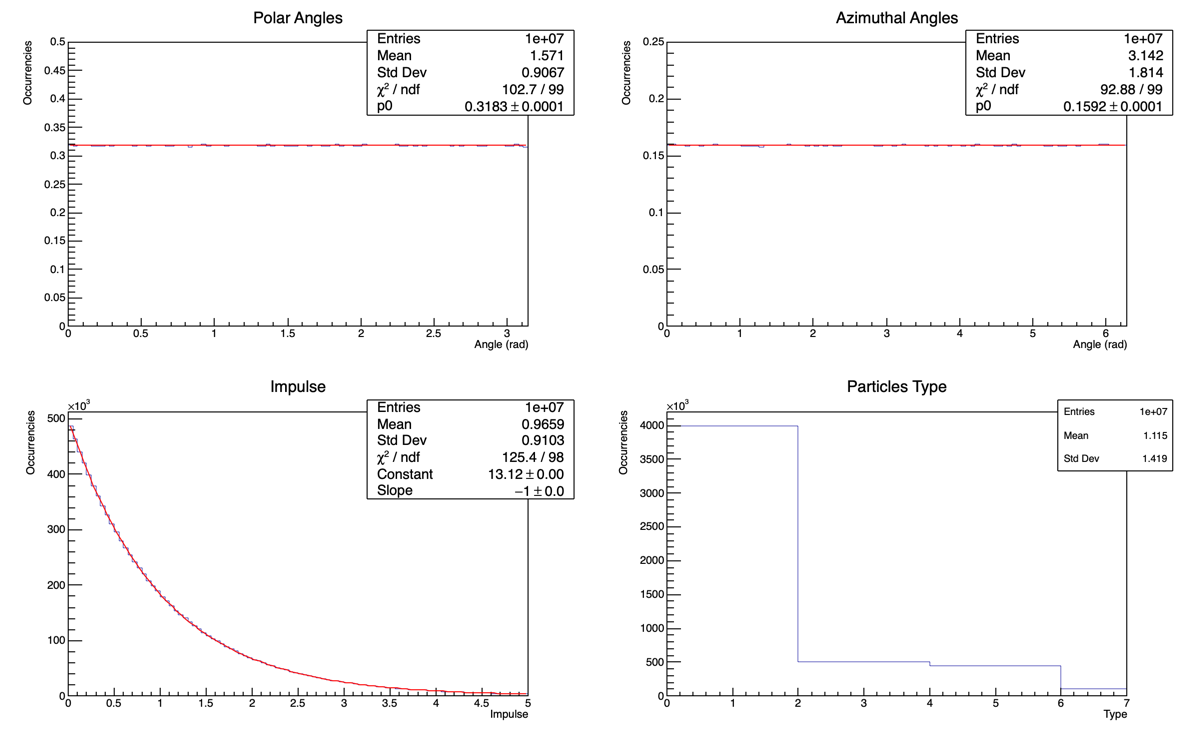
\includegraphics[scale=0.4]{images/DistributionsCanvas.png}

\label{fig:fig1}
\caption{Distribuzioni di angolo polare, angolo azimutale, modulo dell'impulso e tipo di particella}
\end{figure}

\begin{figure}[H]
\centering
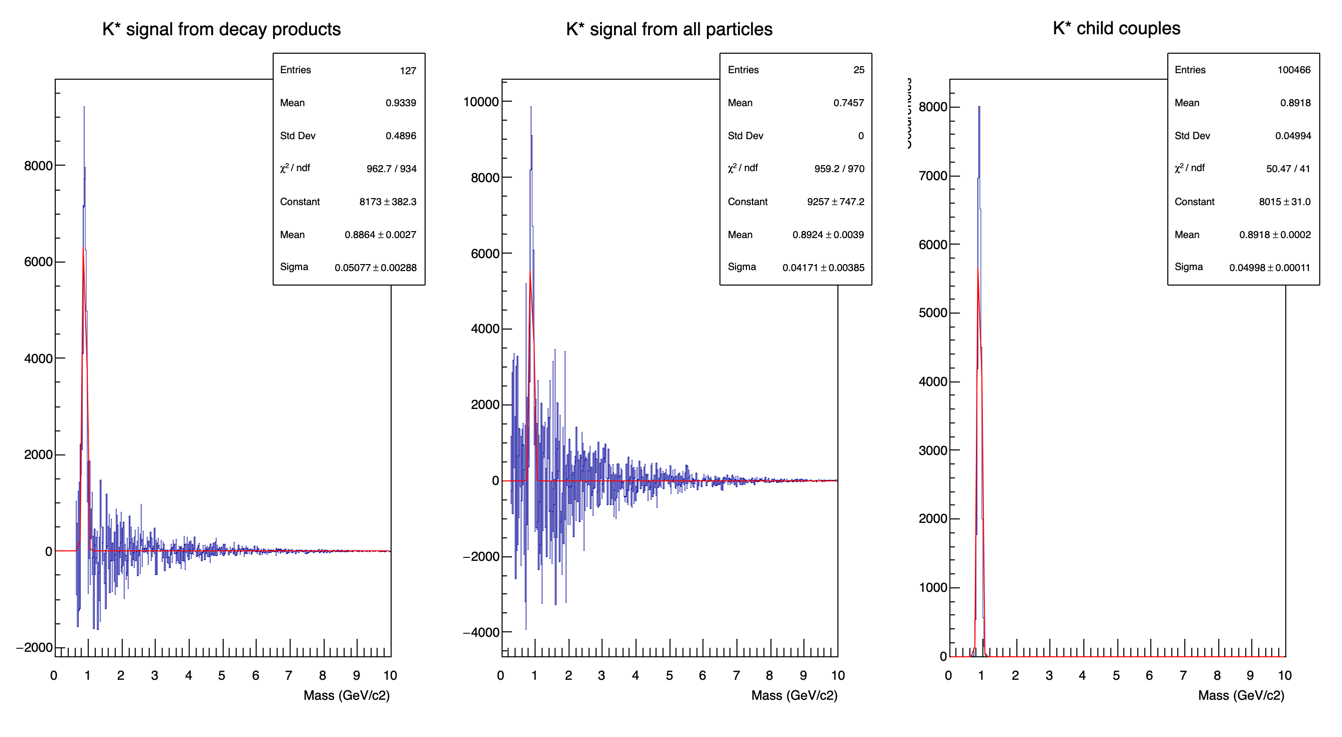
\includegraphics[scale=0.4]{images/SignalCanvas.png}

\label{fig:fig2}
\caption{Distribuzione delle masse invarianti.}
\end{figure}

In figura 2 sono riportate le distribuzioni di massa invariante. A sinistra, ottenute per sottrazione degli istogrammi di massa invariante Pioni-Kaoni \textit{discorde-concorde}. Al centro, ottenuti per sottrazione degli istogrammi di massa invariante tra tutte le particelle di carica \textit{discorde-concorde}. A destra, le masse invarianti ottenute a partire dalle particelle figlie di una stessa K*.

\subsection{Consistenza delle distribuzioni}
Le distribuzioni dei parametri cinematici e del tipo di particella (figura 1) sono consistenti con le impostazioni del generatore. 
I parametri del fit dei segnali estratti della K* e dell'istogramma di benchmark sono consistenti con la massa impostata in fase di generazione. Per quanto riguarda la larghezza di risonanza, si riscontra una piccola differenza per quanto riguarda l'istogramma differenza \textit{Discordi-Concordi} (riga 2 tabella 3).


\section{Appendice}

Riportiamo il codice del programma.

\subsection{Programma di generazione}

\paragraph{main.cpp}

\begin{verbatim}
#include "Definitions.hpp"

#include "TApplication.h"
#include "TDirectory.h"
#include <TH1.h>
#include "TFile.h"

#include "generator/ParticleGenerator.hpp"
#include "particleStorage.hpp"
#include "particles/ParticleType.hpp"

int main(int argc, char **argv) {
    // object ownership setup
    #ifdef PROGRAM_USE_LOCAL_OWNERSHIP
        TDirectory::AddDirectory(kFALSE);
        TH1::AddDirectory(kFALSE);
    #endif

    //allocate memory for particle data
    ResonanceSimulator::ParticleGenerator::loadParticles();

    //create generator object
    ResonanceSimulator::ParticleGenerator generator{};
    // run the simulation
    // save result in unique pointer
    std::unique_ptr<ResonanceSimulator::particleStorage> result{generator(1e5)};

    //write to file
    std::unique_ptr<TFile> output_file{new TFile("Particle.root", "RECREATE")};
    result->Write();
    output_file->Close();

    return 0;
}
\end{verbatim}

\paragraph{Definitions.hpp}
\begin{verbatim}
#ifndef DEFINITIONS_HPP
#define DEFINITIONS_HPP

//HEADER TO DEFINE MACROS FOR THE TEMPLATE CODE

#define APP_NAME "RootProject"
#define PROGRAM_ATTACH_CLING
#define PROGRAM_USE_LOCAL_OWNERSHIP

#ifdef PROGRAM_ATTACH_CLING
#define APP_TYPE TRint
#else
#define APP_TYPE TApplication
#endif

#endif
\end{verbatim}

\paragraph{ParticleType.hpp}

\begin{verbatim}
#ifndef PARTICLETYPE_HPP
#define PARTICLETYPE_HPP

#include <string>

namespace ResonanceSimulator {

    class ParticleType {

    public:
        enum Type { /// particle type enum
            P_Pion, N_Pion, P_Kaon, N_Kaon, P_Prot, N_Prot, R_Kaon
        };
        enum DecaymentType { /// decay result type enum
            P1,//P+ K-
            P2 //P- K+
        };

        ParticleType(int name, double mass, int charge);

        virtual ~ParticleType() = default;

        virtual void Print() const;

        [[nodiscard]] int GetName() const;

        [[nodiscard]] double GetMass() const;

        [[nodiscard]] int GetCharge() const;

        [[nodiscard]] virtual double GetWidth() const;

    private:
        const Type fName; ///name of the particle, expressed as an enum constant
        const double fMass;
        const int fCharge;
    };
}

#endif


\end{verbatim}

\paragraph{ParticleType.cpp}

\begin{verbatim}
#include "particles/ParticleType.hpp"
#include <iostream>

namespace ResonanceSimulator {

    ParticleType::ParticleType(int name, double mass, int charge) :
            fName((Type) name),
            fMass(mass),
            fCharge(charge) {}

    void ParticleType::Print() const {
        std::cout << "Name: " << fName << '\n'
                  << "Mass: " << fMass << '\n'
                  << "Charge: " << fCharge << '\n';
    }

    int ParticleType::GetName() const {
        return fName;
    }

    double ParticleType::GetMass() const {
        return fMass;
    }

    int ParticleType::GetCharge() const {
        return fCharge;
    }

    double ParticleType::GetWidth() const {
        return 0;
    }
}
\end{verbatim}

\paragraph{ResonanceType.hpp}

\begin{verbatim}
#ifndef RESONANCETYPE_HPP
#define RESONANCETYPE_HPP

#include "particles/ParticleType.hpp"

namespace ResonanceSimulator {
    class ResonanceType : public ParticleType {

    public:
        ResonanceType(int name, double mass, int charge, double width);

        [[nodiscard]] double GetWidth() const override;

        void Print() const override;

    private:
        double fWidth;
    };
}

#endif
\end{verbatim}

\paragraph{ResonanceType.cpp}
\begin{verbatim}
#include "particles/ResonanceType.hpp"

#include <iostream>

namespace ResonanceSimulator {

    ResonanceType::ResonanceType(const int name, double mass, int charge, double width) :
            ParticleType{name, mass, charge},
            fWidth{width} {

    }

    double ResonanceType::GetWidth() const {
        return fWidth;
    }

    void ResonanceType::Print() const {
        ParticleType::Print();
        std::cout << "Resonance: " << fWidth << '\n';
    }
}
\end{verbatim}

\paragraph{Particle.hpp}
\begin{verbatim}
#ifndef PARTICLE_HPP
#define PARTICLE_HPP

#include "particles/ParticleType.hpp"
#include "particles/ResonanceType.hpp"

#include <memory>
#include <vector>
#include <string>


namespace ResonanceSimulator {
    class Particle {
        using pTypeStorage = std::vector<std::unique_ptr<ParticleType>>;
    public:
        explicit Particle(int name, double Px = 0, double Py = 0, double Pz = 0);

        [[nodiscard]] int GetParticleName() const;

        static void AddParticleType(int name, double mass, int charge, double width = 0);

        static void PrintParticleList();

        void SetParticleType(int name);

        void PrintData() const;

        void SetP(double px, double py, double pz);

        [[nodiscard]] double GetPx() const;

        [[nodiscard]] double GetPy() const;

        [[nodiscard]] double GetPz() const;

        [[nodiscard]] int GetCharge() const;

        [[nodiscard]] double GetMass() const;

        [[nodiscard]] double GetEnergy() const;

        [[nodiscard]] double InvMass(Particle const &p) const;

        int Decay2body(Particle &dau1, Particle &dau2) const;

    private:
        void Boost(double bx, double by, double bz);

        static pTypeStorage fParticleType;
        static constexpr int fMaxNumParticleType{10};

        int fParticleName;
        double fPx;
        double fPy;
        double fPz;

    };
}

#endif

\end{verbatim}

\paragraph{Particle.cpp}
\begin{verbatim}
#include "particles/Particle.hpp"

#include <algorithm>
#include <iostream>
#include <numeric>
#include <cmath>
#include <cstdlib>

#include "TMath.h"

namespace ResonanceSimulator {

    Particle::Particle(const int name, double Px, double Py, double Pz) :
            fParticleName{name},
            fPx{Px},
            fPy{Py},
            fPz{Pz} {
        //check that the requested particle name exist
        fParticleType.at(name);
    }

    int Particle::GetParticleName() const {
        return fParticleName;
    }

    void Particle::AddParticleType(int name, double mass, int charge, double width) {
        if (fParticleType.size() == fMaxNumParticleType) {
            throw std::runtime_error{"Maximum particle number reached!"};
        }
        //fParticleType.at(name); //se non c'è, inserisci
        if (width == 0) { //may cause troubles with FP numbers
            fParticleType[name] = std::make_unique<ParticleType>(name, mass, charge);
        } else {
            fParticleType[name] = 
            std::make_unique<ResonanceType>(name, mass, charge, width);
        }
    }

    void Particle::SetParticleType(int name) {
        fParticleType.at(name);
        fParticleName = name;
    }

    void Particle::PrintParticleList() {
        std::for_each(fParticleType.cbegin(), fParticleType.cend(), [](auto const &node) {
            node->Print();
        });
    }

    void Particle::PrintData() const {
        std::cout << "Name:" << fParticleName << '\n'
                  << "PX" << fPx << '\n'
                  << "PY" << fPy << '\n'
                  << "PZ" << fPz << '\n';
    }

    void Particle::SetP(double px, double py, double pz) {
        fPx = px;
        fPy = py;
        fPz = pz;
    }

    double Particle::GetPx() const {
        return fPx;
    }

    double Particle::GetPy() const {
        return fPy;
    }

    double Particle::GetPz() const {
        return fPz;
    }

    double Particle::InvMass(const Particle &p) const {
        auto e{GetEnergy() + p.GetEnergy()};

        auto x = fPx + p.GetPx();
        auto y = fPy + p.GetPy();
        auto z = fPz + p.GetPz();

        return TMath::Sqrt(e * e - (x * x + y * y + z * z));

    }

    [[nodiscard]] double Particle::GetMass() const {
        return fParticleType.at(fParticleName)->GetMass();
    }

    double Particle::GetEnergy() const {
        return TMath::Sqrt(TMath::Power(GetMass(), 2) +
                           TMath::Power(fPx, 2) +
                           TMath::Power(fPy, 2) +
                           TMath::Power(fPz, 2));
    }

    //initialise map
    Particle::pTypeStorage Particle::fParticleType(120);

    int Particle::Decay2body(Particle &dau1, Particle &dau2) const {
        if (GetMass() == 0.0) {
            std::cout << "there is no decay if mass is zero";
            return 1;
        }

        double massMot = GetMass();
        double massDau1 = dau1.GetMass();
        double massDau2 = dau2.GetMass();

        double x1, x2, w, y1;

        double invnum = 1. / RAND_MAX;
        do {
            x1 = 2.0 * rand() * invnum - 1.0;
            x2 = 2.0 * rand() * invnum - 1.0;
            w = x1 * x1 + x2 * x2;
        } while (w >= 1.0);

        w = sqrt((-2.0 * log(w)) / w);
        y1 = x1 * w;

        massMot += fParticleType[fParticleName]->GetWidth() * y1;

        if (massMot < massDau1 + massDau2) {
            std::cout << "Decayment cannot be preformed 
            because mass is too low in this channel\n";
            return 2;
        }

        double pout = sqrt(
        (massMot * massMot - (massDau1 + massDau2) * (massDau1 + massDau2)) 
        * (massMot * massMot - (massDau1 - massDau2) * (massDau1 - massDau2))) /
         massMot * 0.5;

        double norm = 2 * M_PI / RAND_MAX;

        double phi = rand() * norm;
        double theta = rand() * norm * 0.5 - M_PI / 2.;
        
        dau1.SetP(pout * sin(theta) * cos(phi), 
        pout * sin(theta) * sin(phi), pout * cos(theta));
        
        dau2.SetP(-pout * sin(theta) * cos(phi),
         -pout * sin(theta) * sin(phi), -pout * cos(theta));

        double energy = sqrt(fPx * fPx + fPy * fPy + fPz * fPz + massMot * massMot);

        double bx = fPx / energy;
        double by = fPy / energy;
        double bz = fPz / energy;

        dau1.Boost(bx, by, bz);
        dau2.Boost(bx, by, bz);

        return 0;
    }


    void Particle::Boost(double bx, double by, double bz) {
        double energy = GetEnergy();

        //Boost this Lorentz vector
        double b2 = bx * bx + by * by + bz * bz;
        double gamma = 1.0 / sqrt(1.0 - b2);
        double bp = bx * fPx + by * fPy + bz * fPz;
        double gamma2 = b2 > 0 ? (gamma - 1.0) / b2 : 0.0;

        fPx += gamma2 * bp * bx + gamma * bx * energy;
        fPy += gamma2 * bp * by + gamma * by * energy;
        fPz += gamma2 * bp * bz + gamma * bz * energy;
    }

    int Particle::GetCharge() const {
        return fParticleType[fParticleName]->GetCharge();
    }

}
\end{verbatim}


\paragraph{ProportionGenerator.hpp}
Questa classe è un template, quindi interamente definita nell'header.

\begin{verbatim}
#ifndef PROPORTIONGENERATOR_HPP
#define PROPORTIONGENERATOR_HPP

#include "particles/ParticleType.hpp"
#include <map>
#include <vector>
#include <iostream>
#include <numeric>

#include "TRandom.h"

namespace ResonanceSimulator {

/**
 * This class generates, based on definite proportions, the elements it is instructed to
 * @tparam GEN The type of the object to be generated
 *
 * NOTE: probability is given in percentile in integer values (to avoid FP problems)
 */
    template<typename GEN>
    class ProportionGenerator {
        /**
         * Struct representing a node of generation, holding values with cumulative weight
         */
        struct Node {
            GEN fValue{}; /// Value
            float fCumulativeProbability{}; ///Relevant cumulative probability
        };
        /**
         * Construct the generator
         * @param sourceData Map associating values to be generated to relevant probability values
         */
    public:
        using probType = float;/// type to represent probability

        explicit ProportionGenerator(std::map<GEN, probType> sourceData) :
                fNodes{} {
            //check probability
            auto totalProb = std::accumulate(sourceData.begin(),
                                             sourceData.end(),
                                             0, [](auto const &acc, auto const &node) {
                        return acc + node.second; //sum probabilities
                    });

            if (std::abs(totalProb - 100) < 0.01) { //FP epsilon
                throw std::runtime_error{"Sum of probability is not 100!"};
            }

            //allocate space for the nodes
            fNodes.reserve(sourceData.size());
            //fill f nodes
            probType accumulator{0}; //hold accumulate probability
            for (auto const &node: sourceData) {
                accumulator += node.second; //accumulate probabilities
                fNodes.push_back({node.first, accumulator});
            }
        }

        /**
         * Generate function
         * @return A randomly generated value, based on the input data
         */
        GEN operator()() {
            //genrate value, cast to int
            probType y{static_cast<probType>(gRandom->Rndm())};

            for (auto const &node: fNodes) {
                //if the value generated is less than, i am generated
                if (y < node.fCumulativeProbability) {
                    return node.fValue; //end cycle
                }
            }
            throw std::runtime_error{"Cannot generate!"};
        }

    private:
        std::vector<Node> fNodes;


    };

}


#endif


\end{verbatim}

\paragraph{ParticleGenerator.hpp}

\begin{verbatim}
#ifndef PARTICLEGENERATOR_HPP
#define PARTICLEGENERATOR_HPP

#include "TRandom3.h"
#include "generator/ProportionGenerator.hpp"
#include "particles/Particle.hpp"

#include "particleStorage.hpp"

#include <deque>

namespace ResonanceSimulator {

    /**
     * This class encapsulates particle generation,
      decayment processing, 
      invariant masses distributions
     */
    class ParticleGenerator {
        using randGen = TRandom3; /// type to be used as random generator
        using PTypeList = ParticleType::Type; /// alias to list of possible particle types
        using PTDecayList = ParticleType::DecaymentType; ///alias to list of 
        // possible decayments
        using PStorage = std::deque<Particle>;

    public:
        explicit ParticleGenerator(unsigned seed = 0);

        /**
         * Register particle list into particle container
         * Data is hard-coded
         */
        static void LoadParticles();

        /**
         * Run the simulation
         * @param NEvents Number of dacyment events to be processed
         * @param NParticlesPerEvent Number of paarticles to be generated per event
         * @return A pointer to a data structure holding the result of the generation
         *
         * Note: the returned pointer's structure is dynamically allocated 
         * and you are responsible
         * for its lifetime management. Consider storing it in a smart pointer.
         */
        ParticleStorage *operator()(unsigned NEvents = 1e5, 
        unsigned NParticlesPerEvent = 1e2);

    private:
        //helper functions
        /**
         * Helper function used to better ecapsulate the particle generation
         * @param EventParticles Reference to the container of generated particles
         * @param DecayProducts Reference to the container of the decay products
         * @param dataStorage Struct holding histograms
         */
        static void CalculateInvariantMass(PStorage const &EventParticles,
                                           PStorage const &DecayProducts,
                                           ParticleStorage &dataStorage) ;

        randGen fRandom; /// Random generator
        ProportionGenerator<PTypeList> fParticleGen;
        ProportionGenerator<PTDecayList> fDecaymentGen;

        static bool IsSameCharge(const Particle &p, const Particle &p2);

        static bool CheckConcordantDecayCouples(const PTypeList &p1_name, 
        const PTypeList &p2_name);

        static bool CheckDiscordantDecayCouples(const PTypeList &p1_name, 
        const PTypeList &p2_name);
    };

} // ResonanceSimulator

#endif 

\end{verbatim}

\paragraph{ParticleGenerator.cpp}

\begin{verbatim}
#include "generator/ParticleGenerator.hpp"

#include "particles/Particle.hpp"
#include "particleStorage.hpp"

#include "TMath.h"

#include "TFile.h"

namespace ResonanceSimulator {
    void ParticleGenerator::LoadParticles() {
        Particle::AddParticleType(PTypeList::P_Pion , 0.13957, 1);
        Particle::AddParticleType(PTypeList::N_Pion, 0.13957, -1);
        Particle::AddParticleType(PTypeList::P_Kaon, 0.49367, 1);
        Particle::AddParticleType(PTypeList::N_Kaon, 0.49367, -1);
        Particle::AddParticleType(PTypeList::P_Prot, 0.93827, 1);
        Particle::AddParticleType(PTypeList::N_Prot, 0.93827, -1);
        Particle::AddParticleType(PTypeList::R_Kaon, 0.89166, 0, 0.050);
    }

    ParticleGenerator::ParticleGenerator(unsigned int seed) :
            fRandom{seed},
            fParticleGen{{
                                 {PTypeList::P_Pion, 0.4},
                                 {PTypeList::N_Pion, 0.4},
                                 {PTypeList::P_Kaon, 0.05},
                                 {PTypeList::N_Kaon, 0.05},
                                 {PTypeList::P_Prot, 0.045},
                                 {PTypeList::N_Prot, 0.045},
                                 {PTypeList::R_Kaon, 0.01}}
            },
            fDecaymentGen{{
                                  {PTDecayList::P1, 0.5},
                                  {PTDecayList::P2, 0.5}
                          }
            } {

    }

    ParticleStorage *ParticleGenerator::operator()(unsigned int NEvents, 
    unsigned int NParticlesPerEvent) {
        //save into particlestorage
        std::unique_ptr<ParticleStorage> dataStorage{new ParticleStorage{}};
        //create default histograms
        ParticleStorage::MakeDefaultHistograms(*dataStorage);
        //Particle type
        PStorage EventParticles{};
        PStorage DecayProducts{};
        //run simulation
        for (unsigned int j = 0; j < NEvents; ++j) {
            //genero le 100 particelle
            for (unsigned int i = 0; i < NParticlesPerEvent; ++i) {
                //generate angles and pulse
                const double phi{gRandom->Uniform(0, 2 * TMath::Pi())};
                const double theta{gRandom->Uniform(0, TMath::Pi())};
                const double P{gRandom->Exp(1)};
                //add values to test histograms (must be done here)
                //because they are not tracked afterwards
                dataStorage->AzimuthalAngles.Fill(phi);
                dataStorage->PolarAngles.Fill(theta);
                dataStorage->Impulse.Fill(P);

                //generate particle
                const PTypeList name{fParticleGen()};
                //add to histogram - try to move in another phase
                dataStorage->ParticlesType.Fill(name);

                //if it is a resonance, make it decay
                if (name == PTypeList::R_Kaon) {
                    //generate decayment pair
                    PTypeList name1{}, name2{};

                    //generate decayment couple
                    if (fDecaymentGen() == PTDecayList::P1) {
                        name1 = PTypeList::P_Pion;
                        name2 = PTypeList::N_Kaon;
                    } else {
                        name1 = PTypeList::N_Pion;
                        name2 = PTypeList::P_Kaon;
                    }

                    Particle p1(name1, 0, 0, 0);
                    Particle p2(name2, 0, 0, 0);
                    Particle pRes(PTypeList::R_Kaon, 
                      P * TMath::Sin(theta) * TMath::Cos(phi),
                      P * TMath::Sin(theta) * TMath::Sin(phi), 
                      P * TMath::Cos(theta));

                    if (pRes.Decay2body(p1, p2) != 0) {
                        throw std::runtime_error("Decay2body failed!");
                    }
                    DecayProducts.push_back(p1);
                    DecayProducts.push_back(p2);
                    //add separately
                    EventParticles.push_back(p1);
                    EventParticles.push_back(p2);
                } else {
                    ResonanceSimulator::Particle p(name, 
                    P * TMath::Sin(theta) * TMath::Cos(phi),
                        P * TMath::Sin(theta) * TMath::Sin(phi), 
                        P * TMath::Cos(theta));
                        
                    EventParticles.push_back(p);
                    
                    
                    //store transverse impulse and energy
                    const double TransImp = std::sqrt(std::pow(p.GetPx(), 2) 
                    + std::pow(p.GetPy(), 2));
                    
                    dataStorage->TransverseImpulse.Fill(TransImp);
                    dataStorage->Energies.Fill(p.GetEnergy());
                }
            }
            CalculateInvariantMass(EventParticles, DecayProducts, *dataStorage);

            EventParticles.clear();
            DecayProducts.clear();
        }

        //release ownership on object and return raw pointer
        return dataStorage.release();

    }

    void ParticleGenerator::CalculateInvariantMass(const PStorage &EventParticles,
                                                   const PStorage &DecayProducts,
                                                   ParticleStorage &dataStorage) {

        //loop throught the dataset, comparing each particle with the others
        for (unsigned int i = 0; i < EventParticles.size(); ++i) {
            auto const &p = EventParticles[i];
            for (unsigned int k = i+1; k < EventParticles.size(); ++k) {
                auto const &p2{EventParticles[k]};
                auto invMass{p.InvMass(p2)};

                PTypeList p1_name{static_cast<PTypeList>(p.GetParticleName())};
                PTypeList p2_name{static_cast<PTypeList>(p2.GetParticleName())};

                //invariant mass between all particles
                dataStorage.InvariantMasses.Fill(invMass);

                //invariant mass depending on charge

                //concordant charge
                if (IsSameCharge(p, p2)) {
                    dataStorage.InvariantMassesAllc.Fill(invMass);

                    //check that the particle couple is of the decay product type
                    if (CheckConcordantDecayCouples(p1_name, p2_name)) {
                        dataStorage.InvariantMassesDecayC.Fill(invMass);
                    }
                }
                    //discordant charge
                else /*if(!IsSameCharge(p, p2))*/{
                    dataStorage.InvariantMassesAlld.Fill(invMass);

                    if (CheckDiscordantDecayCouples(p1_name, p2_name)) {
                        dataStorage.InvariantMassesDecayD.Fill(invMass);
                    }
                }

            }
        }
        //generate invariant mass for decay products
        //since they are inserted in pair after each decay
        //taking 2 each time ensures invariant mass is computed only for children
        //of the same unstable particle
        for (unsigned int i = 0; i < DecayProducts.size(); i += 2) {
            auto &p = DecayProducts[i];
            dataStorage.InvariantMassesDprod.Fill(p.InvMass(DecayProducts[i + 1]));
        }
    }

    bool ParticleGenerator::CheckDiscordantDecayCouples(const PTypeList &p1_name,
                                                        const PTypeList &p2_name) {
        if (p1_name == PTypeList::P_Pion) {
            if (p2_name == PTypeList::N_Kaon) {
                return true;
            }
        } else if (p1_name == PTypeList::P_Kaon) {//symmetric: Kaon+/Pion+
            if (p2_name == PTypeList::N_Pion) {
                return true;
            }
        }
        //same with negative
        if (p1_name == PTypeList::N_Pion) {
            if (p2_name == PTypeList::P_Kaon) {
                return true;
            }
        } else if (p1_name == PTypeList::N_Kaon) {//symmetric: Kaon+/Pion+
            if (p2_name == PTypeList::P_Pion) {
                return true;
            }
        }
        return false;
    }

    bool ParticleGenerator::CheckConcordantDecayCouples(const PTypeList &p1_name,
                                                        const PTypeList &p2_name) {
                                                        //decay product check
//Pion+ / Kaon +
        if (p1_name == PTypeList::P_Pion) {
            if (p2_name == PTypeList::P_Kaon) {
                return true;
            }
        } else if (p1_name == PTypeList::P_Kaon) {//symmetric: Kaon+/Pion+
            if (p2_name == PTypeList::P_Pion) {
                return true;
            }
        }
        //same with negative
        if (p1_name == PTypeList::N_Pion) {
            if (p2_name == PTypeList::N_Kaon) {
                return true;
            }
        } else if (p1_name == PTypeList::N_Kaon) {//symmetric: Kaon+/Pion+
            if (p2_name == PTypeList::N_Pion) {
                return true;
            }
        }
        return false;
    }

    bool ParticleGenerator::IsSameCharge(const Particle &p, const Particle &p2) {
        return (p.GetCharge() * p2.GetCharge()) > 0;
    }


} // ResonanceSimulator
\end{verbatim}

\subsection{Programma di analisi}

\paragraph{analyser.cpp}

\begin{verbatim}
#include "TApplication.h"
#include "TRint.h"
#include "particleAnalyser.hpp"
#include "analyserGraphics.hpp"
#include "TF1.h"
#include "TStyle.h"
#include "TROOT.h"
#include <iostream>

#include "Definitions.hpp"

int main(int argc, char **argv) {    //create root application
    APP_TYPE app(APP_NAME, &argc, argv);

    //create the logic objects
    ResonanceSimulator::dataAnalyser analyser("Particle.root");

    //set style
    //gStyle->SetHistFillColor(kGreen);
    //gStyle->SetHistLineColor(kRed);
    gStyle->SetOptStat(1110);
    gStyle->SetOptFit(111);
    gROOT->ForceStyle(true);

    //do stuff
    ResonanceSimulator::AnalyzerGraphics interface{analyser};

    //draw all canvases
    interface.DrawCanvases();

    //notify that canvas have been drawn
    interface.GraphicSetup();

    //write histograms to file
    interface.WriteHistograms();

    interface.PrintFitResult();

    //run application
    app.Run();
    return 0;
}
\end{verbatim}

\paragraph{analyserGraphics.hpp}

\begin{verbatim}
#ifndef ANALYSERGRAPHICS_HPP
#define ANALYSERGRAPHICS_HPP

#include <memory>
#include <unordered_map>
#include <vector>

#include "TCanvas.h"
#include "TPad.h"
#include "TLegend.h"

#include "particleAnalyser.hpp"

namespace ResonanceSimulator {
    /**
     * This class encapsulates graphics for the particle data analysis
     */
    class AnalyzerGraphics {
        using CanvasPtr = std::unique_ptr<TCanvas>;
        using CanvasCont = std::unordered_map<std::string,CanvasPtr>;

    public:
        explicit AnalyzerGraphics(DataAnalyser &analyser);

        void GraphicSetup();
        void DrawCanvases();
        void WriteHistograms() const;
        void PrintFitResult() const;

    private:
    /// Pointer to the object handling analysed data
        std::shared_ptr<particleStorage> fInputData; 
        std::shared_ptr<SignalResult> fSignalResult;
        dataAnalyser::GenerationResult fGenerationDistributionFit;

        //canvas with resulting histograms, similar with similar
        CanvasCont fCanvasContainer;

        void PrintSignalFit(std::string const& initialText, 
        const SignalResult::FitPtr &fit) const;
    };
}

#endif 
\end{verbatim}

\paragraph{analyserGraphics.cpp}

\begin{verbatim}
#include "analyserGraphics.hpp"

#include <algorithm>
#include <iostream>

namespace ResonanceSimulator {
    AnalyzerGraphics::AnalyzerGraphics(dataAnalyser &analyser) :
            fInputData{analyser.GetData()}, //get input data
            fSignalResult{analyser.GetDecaymentSignal()}, //run fit
            fGenerationDistributionFit{analyser.GetGenerationFits()},
            fCanvasContainer{}{
        //create canvases
        {
        CanvasPtr MassCanvas{
        new TCanvas("MassCanvas", "Masse Invarianti", 1200, 800)};
        
        CanvasPtr DistributionsCanvas{
        new TCanvas("DistributionsCanvas", "Distribuzioni di generazione", 1200, 800)};
        
        CanvasPtr SumCanvas{
        new TCanvas("SignalCanvas", "Segnali estratti", 1200, 800)};
        
        CanvasPtr DynamicsCanvas{
        new TCanvas("DynamicsCanvas", "Parametri meccanici", 1200, 800)};

        //register canvases
        //split insertion and allocation to avoid duplicating name
        //in subscript operator
        fCanvasContainer[MassCanvas->GetName()] = std::move(MassCanvas);
        fCanvasContainer[DistributionsCanvas->GetName()] = std::move(DistributionsCanvas);
        fCanvasContainer[SumCanvas->GetName()] = std::move(SumCanvas);
        fCanvasContainer[DynamicsCanvas->GetName()] = std::move(DynamicsCanvas);
    }

    }

    void AnalyzerGraphics::WriteHistograms() const {
        for(auto& canvas: fCanvasContainer){
            canvas.second->Print((
                    std::string{canvas.second->GetName()}+".pdf"
                    ).c_str());
            canvas.second->Print((
                                         std::string{canvas.second->GetName()}+".C"
                                 ).c_str());
            canvas.second->Print((
                                         std::string{canvas.second->GetName()}+".root"
                                 ).c_str());
        }

    }

    void AnalyzerGraphics::DrawCanvases() {
        const char *options{"HIST,SAME"};

        //bind references to ptr for simplicity
        CanvasPtr& MassCanvas{fCanvasContainer["MassCanvas"]};
        CanvasPtr& DistributionsCanvas{fCanvasContainer["DistributionsCanvas"]};
        CanvasPtr& SignalCanvas{fCanvasContainer["SignalCanvas"]};
        CanvasPtr& DynamicsCanvas{fCanvasContainer["DynamicsCanvas"]};

        //invariant masses
        MassCanvas->Divide(3, 2);

        MassCanvas->cd(1);
        fInputData->InvariantMasses.Draw(options);
        MassCanvas->cd(2);
        fInputData->InvariantMassesAllc.Draw(options);
        MassCanvas->cd(3);
        fInputData->InvariantMassesAlld.Draw(options);
        MassCanvas->cd(4);
        fInputData->InvariantMassesDecayC.Draw(options);
        MassCanvas->cd(5);
        fInputData->InvariantMassesDecayD.Draw(options);
        MassCanvas->cd(6);
        fInputData->InvariantMassesDprod.Draw(options);

        //generation distributions
        //fix scale on polar/azimuth distributions
        fInputData->PolarAngles.GetYaxis()->SetRangeUser(0,0.5);
        fInputData->AzimuthalAngles.GetYaxis()->SetRangeUser(0,0.25);

        DistributionsCanvas->Divide(2, 2);
        DistributionsCanvas->cd(1);
        fInputData->PolarAngles.Draw(options);
        fGenerationDistributionFit["Polar"].Draw("SAME");

        DistributionsCanvas->cd(2);
        fInputData->AzimuthalAngles.Draw(options);
        fGenerationDistributionFit["Azimuth"].Draw("SAME");

        DistributionsCanvas->cd(3);
        fInputData->Impulse.Draw(options);
        fGenerationDistributionFit["Pulse"].Draw("SAME");

        DistributionsCanvas->cd(4);
        fInputData->ParticlesType.Draw(options);

        //signal canvas
        SignalCanvas->Divide(3, 1);
        SignalCanvas->cd(1);
        fSignalResult->signal1->Draw(options);

        fSignalResult->fitSignal1.Draw("SAME");
        SignalCanvas->cd(2);
        fSignalResult->signal2->Draw(options);

        fSignalResult->fitSignal2.Draw("SAME");
        SignalCanvas->cd(3);
        fInputData->InvariantMassesDprod.Draw(options);
        fSignalResult->fitSignal3.Draw("SAME");

        //mechanical canvas
        DynamicsCanvas->Divide(2, 1);

        DynamicsCanvas->cd(1);
        fInputData->TransverseImpulse.Draw(options);
        DynamicsCanvas->cd(2);
        fInputData->Energies.Draw(options);
    }

    void AnalyzerGraphics::GraphicSetup() {
        for(auto& canvas: fCanvasContainer){
            canvas.second->Modified();
            canvas.second->Update();
        }
    }

    void AnalyzerGraphics::PrintFitResult() const {
        auto const& genFit{fGenerationDistributionFit};

        auto const& polar{genFit.at("Polar")};
        auto const& azimuth{genFit.at("Azimuth")};
        auto const& impulse{genFit.at("Pulse")};
        //Print distribution fit
        std::cout<<"=========== DISTRIBUTION FIT RESULT ===============\n";

        std::cout<<"Impulse: \n"<<"Constant: "<<impulse.GetParameter(0)<<"\n"
            <<"Slope: "<<impulse.GetParameter(1)<<"\n"
            <<"Chi/Dof: "<<impulse.GetChisquare()/impulse.GetNDF()<<"\n";

        std::cout<<"=============\n";

        std::cout<<"Azimuthal angle: \n"<<"Constant: "<<azimuth.GetParameter(0)<<"\n"
            <<"Chi/Dof: "<<azimuth.GetChisquare()/azimuth.GetNDF()<<"\n";

        std::cout<<"=============\n";

        std::cout<<"Polar angle: \n"<<"Constant: "<<polar.GetParameter(0)<<"\n"
                 <<"Chi/Dof: "<<polar.GetChisquare()/polar.GetNDF()<<"\n";

        std::cout<<"=============\n";

        auto const& discordantPK{fSignalResult->fitSignal1};
        auto const& discordantALL{fSignalResult->fitSignal2};
        auto const& benchmark{fSignalResult->fitSignal3};

        std::cout<<"============K* SIGNAL FITS===========\n";

        PrintSignalFit("Discordant Pion-Kaon", discordantPK);
        PrintSignalFit("All discordant",discordantALL);
        PrintSignalFit("Benchmark",benchmark);
    }

    void AnalyzerGraphics::PrintSignalFit(std::string const& initialText, 
    const SignalResult::FitPtr &fit) const {
    
        std::cout << initialText<<"\n" << "Constant: " << 
        fit.GetParameter(0) << " +/- "<<fit.GetParError(0) << "\n"
        
                  << "Mass (mean): " << fit.GetParameter(1) <<
                   " +/- "<<fit.GetParError(1)<<"\n"
                   
                  << "Resonance width (sigma): " << fit.GetParameter(2)
                  << " +/- "<<fit.GetParError(2) << "\n"
                  << "Chi/Dof: " <<fit.GetChisquare()/fit.GetNDF() << "\n";

        std::cout<<"=============\n";
    }
}

\end{verbatim}

\paragraph{particleAnalyser.hpp}

\begin{verbatim}
#ifndef PARTICLEAANALYSER_HPP
#define PARTICLEAANALYSER_HPP

#include "TFile.h"
#include "TH1.h"
#include <string>
#include <unordered_map>

#include "particleStorage.hpp"
#include "dataStructures/signalFitResult.hpp"

namespace ResonanceSimulator {
    /**
     * This class encapsulates the data analysis for the K* decayment trace.
     * The class acts as a mere analysis running tool: 
     *results are NOT stored internally. The user is required
     * to handle their storage
     *
     * The class provides shared ownership about source data, to allow further
     * manipulation before running the true analysis
     */
    class DataAnalyser {

    public:
        using dataContainer = ParticleStorage;
        using dataContainerPtr = std::shared_ptr<dataContainer>;
        using dataContainerConstPtr = std::shared_ptr<const dataContainer>;
        using GenerationResult = std::unordered_map<std::string, TF1>;
        /**
         * Construct the analyser class
         * @param path Path to the ROOT file holding the required objects
         */
        explicit DataAnalyser(std::string const &path);

        /**
         * Get a const reference to underlying dataContainer structure
         */
        [[nodiscard]] dataContainerPtr GetData();

        /**
        * Get a const pointer to underlying dataContainer structure
        */
        [[nodiscard]] dataContainerConstPtr GetData() const;


        /**
         * Run the decayment signal analysis
         * @return A shared pointer to SignalResult structure holding K* 
         *decayment signal distribution along
         * with gaussian fit results
         *
         * Note: the returned structure is generated ex-novo at each invocation. 
         *Nothing is stored internally about this analysis result
         */
        [[nodiscard]] std::shared_ptr<SignalResult> GetDecaymentSignal() const;

        /**
         * Fit the histograms of the data used to generate decayment events and particles
         * @return Struct holding fit result data
         */
        [[nodiscard]] GenerationResult GetGenerationFits() const;

    private:
        dataContainerPtr fData; ///Underlying data container
    };
}

#endif 

\end{verbatim}

\paragraph{particleAnalyser.cpp}


\begin{verbatim}
#include "particleAnalyser.hpp"

#include "particleStorage.hpp"
#include "dataStructures/signalFitResult.hpp"

#include "TFitResult.h"
#include "TFitResultPtr.h"

#include <sstream>

namespace ResonanceSimulator {

    DataAnalyser::DataAnalyser(const std::string &path) :
    //create empty TList
            fData{} {
        //open the file in read only mode
        TFile data_source{path.c_str(), "READ"};

        //check that the file was opened correctly
        if (!data_source.IsOpen()) {
            throw std::runtime_error{"Cannot open root file. Path: " + path};
        }

        //load data
        fData = dataContainerPtr{
                dynamic_cast<dataContainer *>(
                data_source.Get("ResonanceSimulator::particleStorage"))
        };
        
        //normalize generation distirbutions
        //for bin width, i chose bin 1 but all bins have the same width
        fData->PolarAngles.Scale(1./
        (fData->PolarAngles.GetEntries()*fData->PolarAngles.GetBinWidth(1)));
        
        fData->AzimuthalAngles.Scale(1./
        (fData->AzimuthalAngles.GetEntries()*fData->AzimuthalAngles.GetBinWidth(1)));
    }

    DataAnalyser::dataContainerPtr DataAnalyser::GetData() {
        return fData;
    }

    DataAnalyser::dataContainerConstPtr DataAnalyser::GetData() const {
        return fData;
    }


    std::shared_ptr<SignalResult> DataAnalyser::GetDecaymentSignal() const {
        auto signal1 = new TH1F{
                fData->InvariantMassesDecayD
                //fData->invMasses["DiscordantPK"]-fData->invMasses["ConcordantPK"]
        };

        signal1->Add(&fData->InvariantMassesDecayC,-1);

        signal1->SetName("DecaySignal1");
        signal1->SetTitle("K* signal from decay products");

        auto signal2 = new TH1F{
                fData->InvariantMassesAlld};
        signal2->Add(&fData->InvariantMassesAllc,-1);

        signal2->SetName("DecaySignal2");
        signal2->SetTitle("K* signal from all particles");

        //run fit
        TF1 fit1{"FIT_SIGNAL_1","gaus",0,10};
        signal1->Fit(&fit1);

        TF1 fit2{"FIT_SIGNAL_2","gaus",0,10};
        signal2->Fit(&fit2);

        TF1 fit3{"FIT_SIGNAL_RAW","gaus",0,10};
        fData->InvariantMassesDprod.Fit(&fit3);
        //return the 2 signals
        return std::make_shared<SignalResult>(signal1, signal2, fit1, fit2, fit3);
    }

    DataAnalyser::GenerationResult DataAnalyser::GetGenerationFits() const {
        //Get angular data
        auto &azimuthal{fData->AzimuthalAngles};
        auto &polar{fData->PolarAngles};
        auto &pulse{fData->Impulse};

        //fit data storage
        GenerationResult fits;

        //run the fit, saving results in tfit ptr
        fits.insert({"Azimuth", TF1{"FIT_AZIMUTH","pol0",0,10}});
        fits.insert({"Polar", TF1{"FIT_POLAR","pol0",0,10}});
        fits.insert({"Pulse", TF1{"FIT_PULSE","expo",0,10}});

        azimuthal.Fit(&fits["Azimuth"]);
        polar.Fit(&fits["Polar"]);
        pulse.Fit(&fits["Pulse"]);

        return fits;
    }

}
\end{verbatim}

\paragraph{particleStorage.hpp}
\begin{verbatim}
#ifndef PARTICLESTORAGE_HPP
#define PARTICLESTORAGE_HPP

#include "TH1.h"
#include "TObject.h"
#include <map>

namespace ResonanceSimulator {
    /**
     * Store datas to be analysed
     * The storage type may vary across different versions
     */
    struct ParticleStorage : public TObject {
        using histCont = std::map<std::string, TH1F>;
        using hist = TH1F;

        ParticleStorage() = default;

        static constexpr unsigned invMassBins{1000};
        static void MakeDefaultHistograms(particleStorage &storage);

        //Histograms classified by type
        //generation histograms
        hist ParticlesType{};
        hist AzimuthalAngles{};
        hist PolarAngles{};
        //dynamics
        hist Impulse{};
        hist TransverseImpulse{};
        hist Energies{};
        //relativistic
        hist InvariantMasses{};
        hist InvariantMassesAlld{};
        hist InvariantMassesAllc{};
        /// Concordant particles that can be generated as result of decay
        hist InvariantMassesDecayC{};
        /// Discordant particles that can be generated as result of decay 
        hist InvariantMassesDecayD{}; 
        hist InvariantMassesDprod{};

    ClassDefOverride(particleStorage, 1);
    };
}

#endif
\end{verbatim}

\paragraph{particleStorage.cpp}
La macro ClassImp è commentata poiché dà errori di compilazone ed è segnalata come deprecata.

\begin{verbatim}
#include "particleStorage.hpp"
#include "TMath.h"

namespace ResonanceSimulator {
    //ClassImp(ParticleStorage);
    
    void ParticleStorage::MakeDefaultHistograms(ParticleStorage &storage) {
        storage.ParticlesType = 
        TH1F("ParticlesType", "Particles Type; Type; Occurrencies"
        , 7, 0, 7);
        
        storage.AzimuthalAngles = 
        TH1F("AzimuthalAngles", "Azimuthal Angles; Angle (rad); Occurrencies",
         100, 0, 2 * TMath::Pi());
        
        storage.PolarAngles = 
        TH1F("PolarAngles", "Polar Angles; Angle (rad); Occurrencies",
         100, 0, TMath::Pi());
        
        storage.Impulse = 
        TH1F("Impulse", "Impulse; Impulse; Occurrencies",
         100, 0, 5);
        
        storage.TransverseImpulse = 
        TH1F("TransverseImpulse", "Transverse Impulse; Impulse; Occurencies",
         100, 0, 5);
        
        storage.Energies = 
        TH1F("Energies", "Energies; Energy (GeV); Occurrencies",
         100, 0, 10);
        
        storage.InvariantMasses = 
        TH1F("InvariantMasses", "Invariant Masses; Mass (GeV/c2); Occurencies",
         100, 0, 10);
        

        storage.InvariantMassesAlld = 
        TH1F("InvariantMassesAlld", "All discordant charges; Mass (GeV/c2); Occurencies",
         invMassBins, 0, 10);
        
        storage.InvariantMassesAllc = 
        TH1F("InvariantMassesAllc", "All concordant charges; Mass (GeV/c2); Occurencies",
         invMassBins, 0, 10);
        
        storage.InvariantMassesDecayC = 
        TH1F("InvariantMassesDecayC", 
        "Pion/Kaon concordant charges; Mass (GeV/c2); Occurencies",
         invMassBins, 0, 10);
        
        storage.InvariantMassesDecayD = 
        TH1F("InvariantMassesDecayD", 
        "Pion/Kaon discordant charges; Mass (GeV/c2); Occurencies",
         invMassBins, 0, 10);
        
        storage.InvariantMassesDprod = 
        TH1F("InvariantMassesDprod", "K* child couples; Mass (GeV/c2); Occurencies",
         invMassBins, 0, 10);

        //enable error propagation for histograms
        storage.InvariantMassesAlld.Sumw2();
        storage.InvariantMassesAllc.Sumw2();
        storage.InvariantMassesDecayC.Sumw2();
        storage.InvariantMassesDecayD.Sumw2();
    }
}
\end{verbatim}

\paragraph{dataStructures/SignalFitResult.hpp}

\begin{verbatim}
#ifndef SIGNALFITRESULT_HPP
#define SIGNALFITRESULT_HPP

#include "TH1.h"
#include "TFitResultPtr.h"
#include "TF1.h"

#include <memory>

namespace ResonanceSimulator {
    /**
 * Struct to hold the result of the required histogram difference
 */
    struct SignalResult {
        using Hist = TH1F*;
        using FitPtr = TF1;

        SignalResult(Hist signal1, Hist signal2, 
        const FitPtr &fitSignal1, const FitPtr &fitSignal2,
                     const FitPtr &fitSignal3);

		/// Difference between the 2 kaon-pion histograms
        Hist signal1;
        /// Difference between the concordant and discordant charge histogram
        Hist signal2; 
        
        FitPtr fitSignal1; /// Fit result ptr for signal 1
        FitPtr fitSignal2; /// Fit result ptr for signal 2
        FitPtr fitSignal3; /// Fit result for direct child histogram


    };

}

#endif
\end{verbatim}

\paragraph{dataStructures/SignalFitResult.cpp}
\begin{verbatim}
#include "Definitions.hpp"

#include "dataStructures/signalFitResult.hpp"

namespace ResonanceSimulator {

    SignalResult::SignalResult(SignalResult::Hist signal1, 
     	SignalResult::Hist signal2,
     	const SignalResult::FitPtr &fitSignal1, 
     	const SignalResult::FitPtr &fitSignal2,
     	const SignalResult::FitPtr &fitSignal3) : 
     signal1(signal1), 
     signal2(signal2),
     fitSignal1(fitSignal1), 
     fitSignal2(fitSignal2),
     fitSignal3(fitSignal3) {}
}
\end{verbatim}

\end{document}